\documentclass[12pt]{article}
\raggedbottom

\usepackage[utf8]{inputenc}
\usepackage{graphicx}
\usepackage[english]{babel}
\usepackage{csquotes}
\usepackage{lipsum}
\usepackage{fancyhdr}
\usepackage{pdfpages}
\usepackage{wrapfig}
\usepackage{siunitx}
\usepackage{subcaption}
\usepackage{float}
\usepackage{enumitem}
\usepackage{subcaption}
\usepackage{framed}
\usepackage{listings,xcolor}
\usepackage{inconsolata}
\usepackage{setspace}
\usepackage[T1]{fontenc}
\usepackage[hidelinks]{hyperref}
\usepackage{booktabs}
\usepackage{amsmath}
\usepackage{csquotes}
\usepackage[backend=biber, sorting=none]{biblatex}
\usepackage[a4paper,width=160mm,top=25mm,bottom=25mm]{geometry}

\captionsetup{compatibility=false}
\definecolor{shadecolor}{gray}{0.8}
\addbibresource{sources.bib}
\setcounter{biburllcpenalty}{7000}
\setcounter{biburlucpenalty}{8000}

\title{\textbf{\textsc{Assignment 4: RAM}}\\Digital Forensics}

\author{Elisa Pioldi\\
        ID 12305812}
\date{January 17, 2024}

\begin{document}

\maketitle

\section{Factual part}

\subsection{Background}

\subsubsection{Case description}

This analysis is divided into two parts: 
\begin{enumerate}
        \item Acquisition and analysis of a choosen RAM dump
        \item Analysis of a RAM dump sent by an unknown source
\end{enumerate}

\subsubsection{Software and hardware specifications}
\label{sec:specs}

For this analysis, I utilized the following software:

\begin{itemize}
    \item \textbf{Volatility} \cite{volatility} -- version 2.5.2; to analyze the RAM dump.
    \item \textbf{WinPmem} \cite{winpmem} to acquire the RAM dump.
\end{itemize}

\subsection{Analysis of the choosen RAM dump}

\subsubsection{Preprocessing and acquisition}

First, I created a virtual machine with Windows 7. To make the image unique, I created a simple application called \textit{digitalForensic} in Powershell and I executed it. 

Then I installed WinPmem and I acquired the RAM dump. The SHA-256 of \texttt{physmem.raw} is:\\
\texttt{32706ABA85866D8FA8726658B223AB497FD5BBFC1E42D53049567680A36078B7}

\subsubsection{Analysis}

Once I acquired the RAM dump, I used Volatility to analyze it. First I listed the processes running at the time of the dump. The results are shown in Figure \ref{fig:pslist}. Then I scanned for processes, as shown in Figure \ref{fig:psscan}.

\begin{figure}
        \centering
        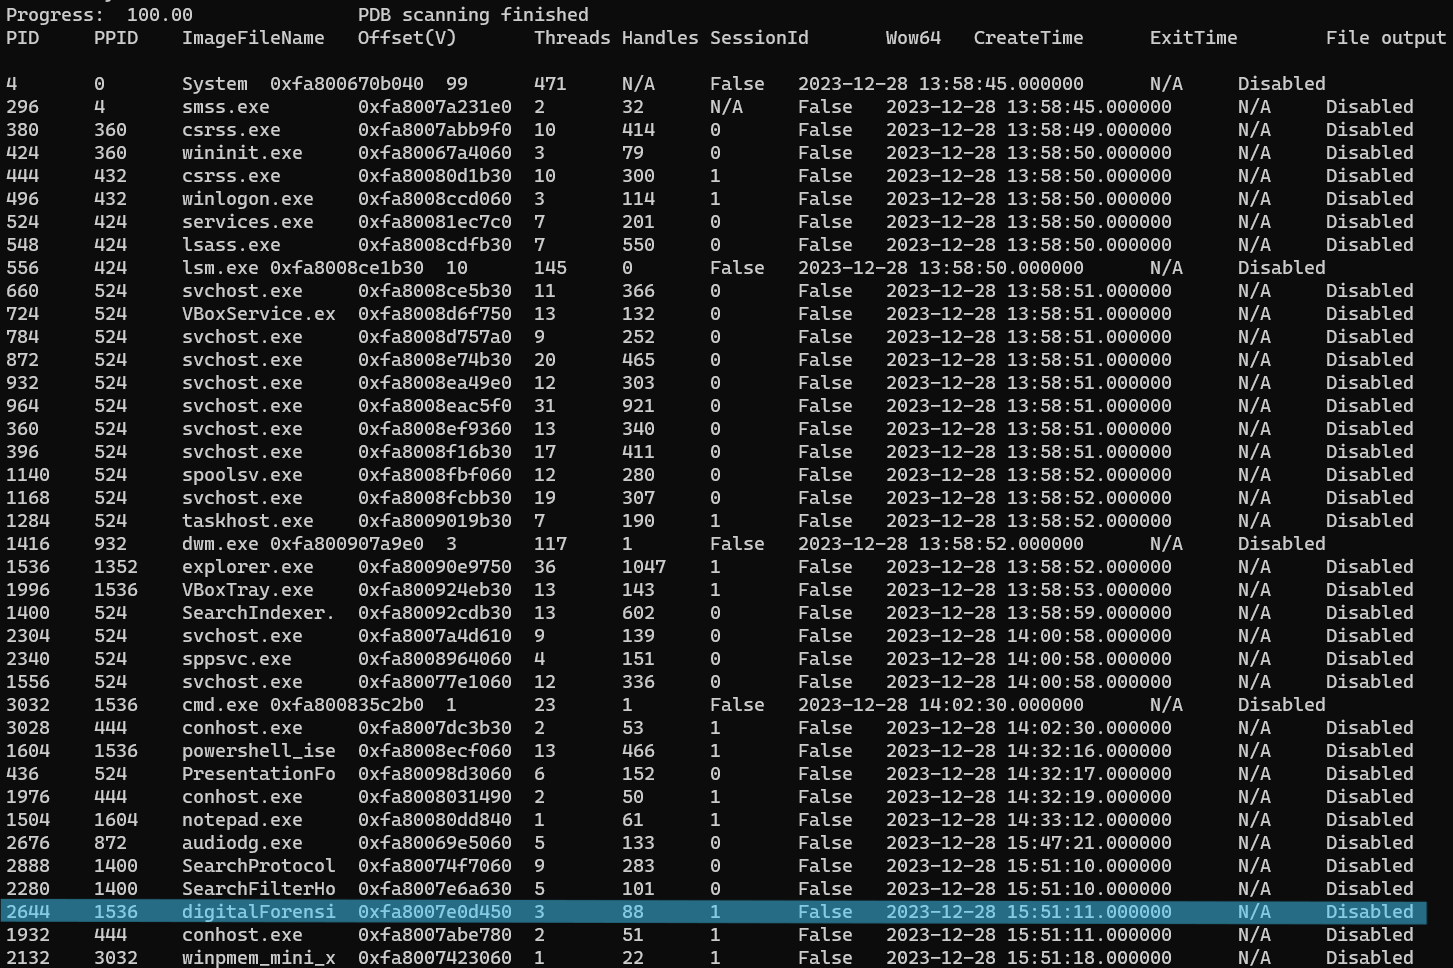
\includegraphics[width=\textwidth]{images/pslist.png}
        \caption{List of processes.}
        \label{fig:pslist}
\end{figure}

\begin{figure}
        \centering
        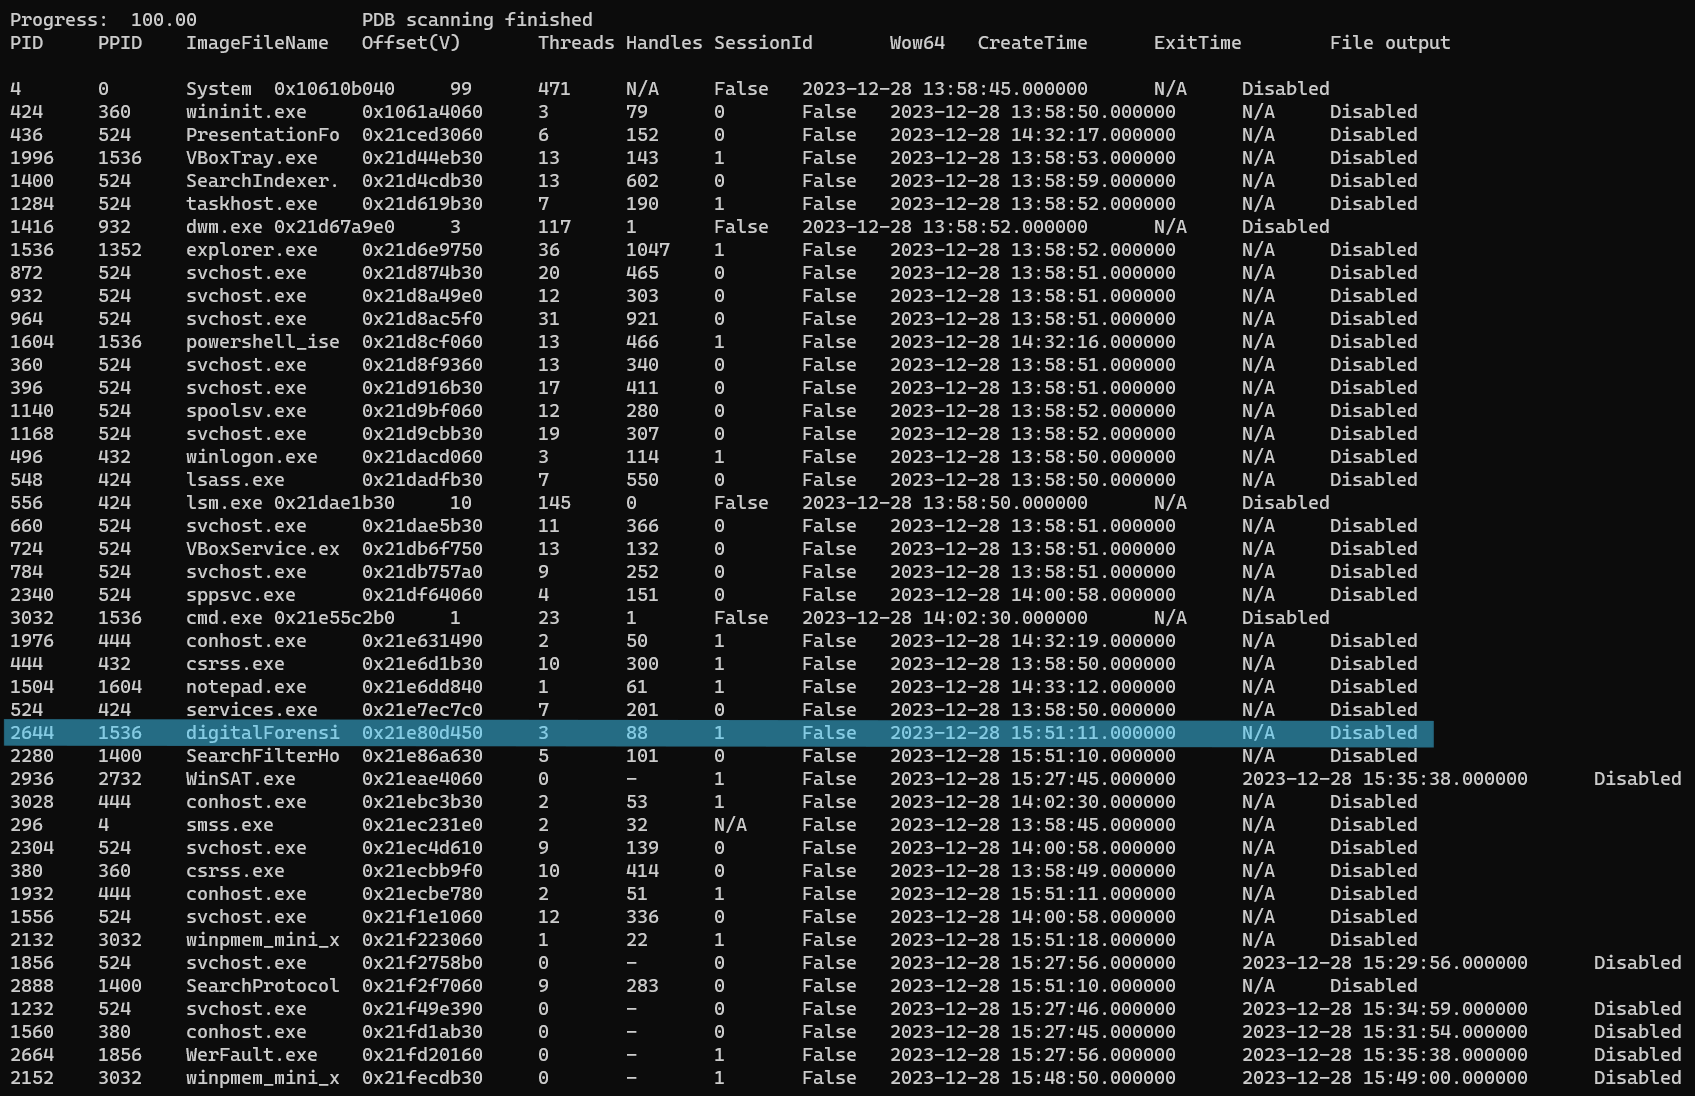
\includegraphics[width=\textwidth]{images/psscan.png}
        \caption{Scanning for processes.}
        \label{fig:psscan}
\end{figure}

You can see highlighted in blue the process \textbf{digitalForensic.exe}, which is the one I created. 

We can notice that scanning and listing processes gives different results. This is because \texttt{pslist} only lists processes that are in the \textit{EPROCESS} structure, while \texttt{psscan} scans the physical memory for the \textit{EPROCESS} structure. This means that \texttt{psscan} can find processes that are not in the \textit{EPROCESS} structure, such as terminated processes. 

Finally, I listed the network connections, as shown in Figure \ref{fig:netscan}.

\begin{figure}
        \centering
        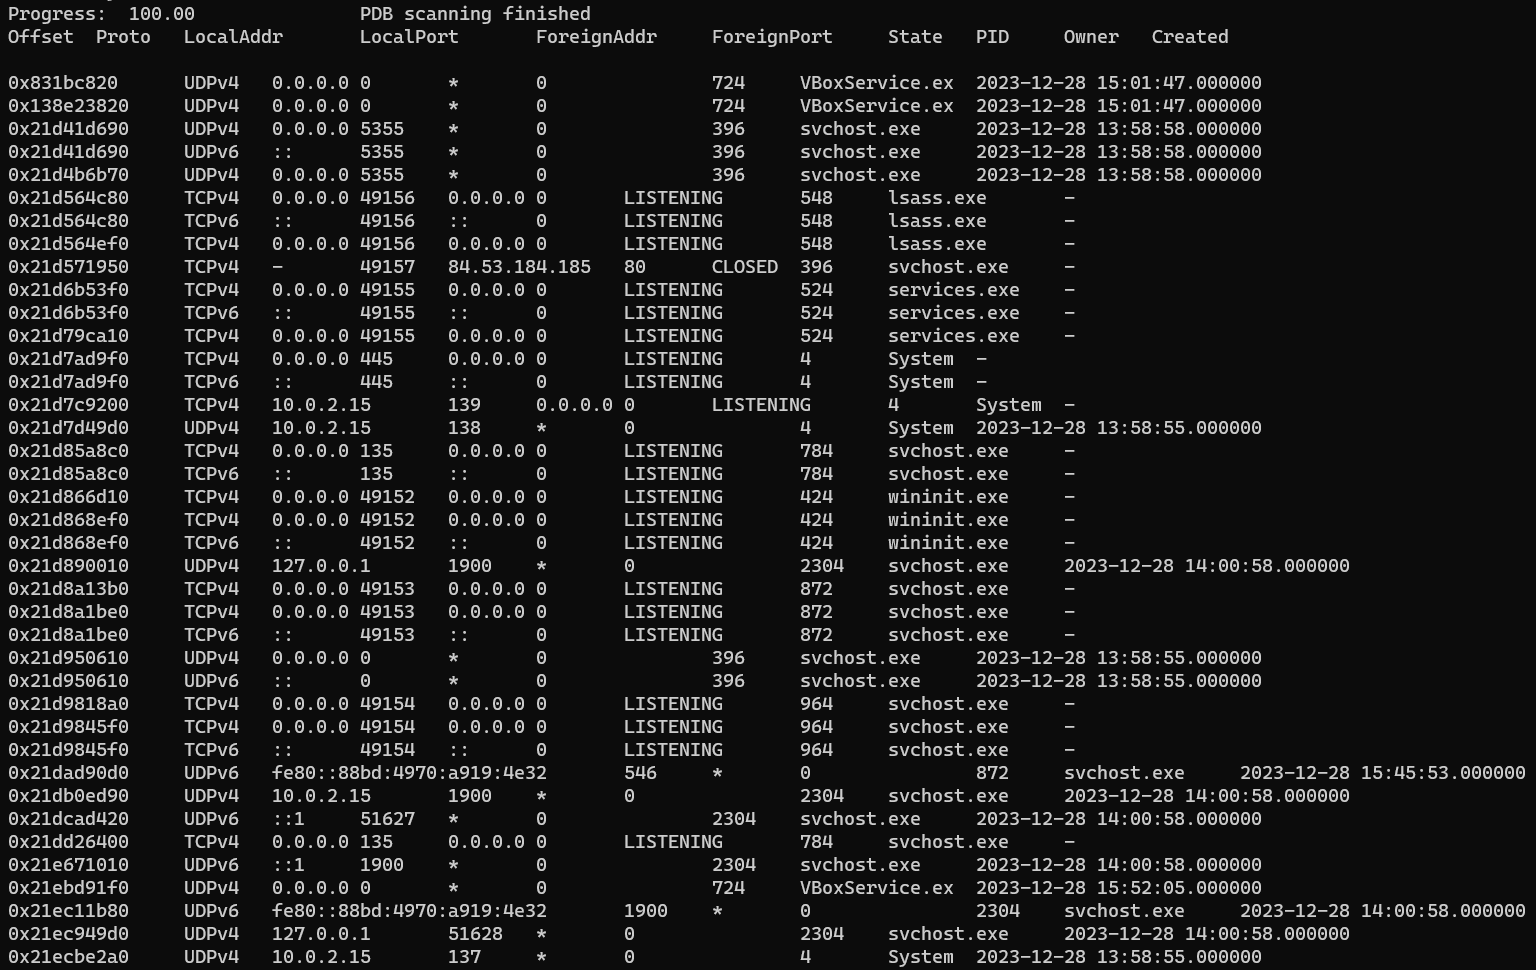
\includegraphics[width=\textwidth]{images/netscan.png}
        \caption{List of network connections.}
        \label{fig:netscan}
\end{figure}


\subsection{Analysis of the unknown RAM dump}

I received a RAM dump from an unknown source. 
The SHA-256 of \texttt{physmem.raw} is:
\texttt{fee4a87527509ed8a67c51a2b3e21a74ae52739e0d69020312180339cfd79e3b}

\subsubsection{Basic information}

First of all, I checked the basic information about the RAM dump, such as the operating system, the architecture, the profile, the time of the dump, etc. The results are shown in Table \ref{table:info}.

\begin{table}[!ht]
        \centering
        \begin{tabular}{ll}
        \toprule
        \textbf{Property} & \textbf{Value} \\
        \midrule
        layer\_name & 0 WindowsIntel32e \\
        memory\_layer & 1 FileLayer \\
        KdVersionBlock & 0xf804216099a0 \\
        Major/Minor & 15.22621 \\
        MachineType & 34404 \\
        KeNumberProcessors & 2 \\
        SystemTime & 2023-01-09 22:17:11 \\
        NtSystemRoot & C:\textbackslash Windows \\
        NtProductType & NtProductWinNt \\
        NtMajorVersion & 10 \\
        NtMinorVersion & 0 \\
        PE MajorOperatingSystemVersion & 10 \\
        PE MinorOperatingSystemVersion & 0 \\
        PE Machine & 34404 \\
        PE TimeDateStamp & Mon Jul  5 20:20:35 2100 \\
        \bottomrule
        \end{tabular}
        \caption{Checksums of important files.}
        \label{table:info}
\end{table}

\subsubsection{Processes}

I looked for the processes running at the time of the dump (you can see some of them in Figure \ref{fig:bobps}):

\begin{figure}
        \centering
        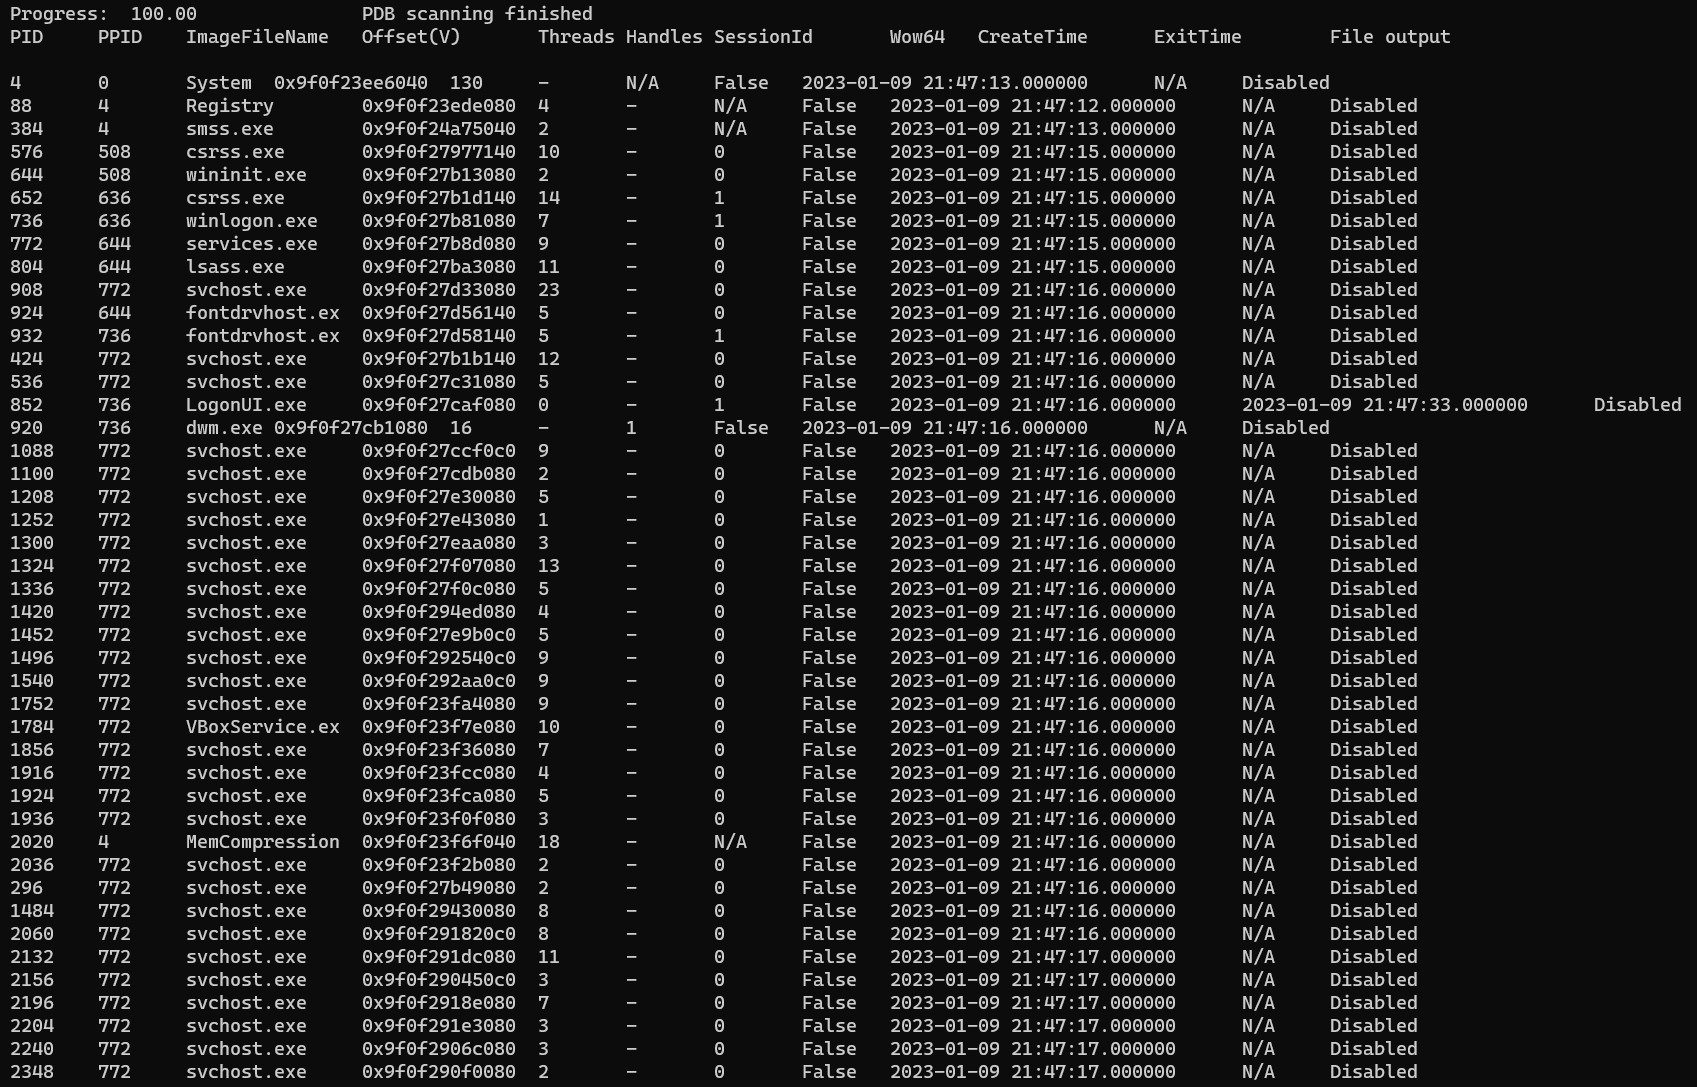
\includegraphics[width=\textwidth]{images/bobps.png}
        \caption{List of processes.}
        \label{fig:bobps}
\end{figure}


\begin{enumerate}
\item \textbf{System} (PID 4)

\item \textbf{Registry} (PID 88)

\item \textbf{smss.exe} (PID 384)

\item \textbf{csrss.exe} (PID 576, 652)

\item \textbf{wininit.exe} (PID 644)

\item \textbf{winlogon.exe} (PID 736)

\item \textbf{services.exe} (PID 772)

\item \textbf{lsass.exe} (PID 804)

\item \textbf{svchost.exe} (PID 908, 424, 536, 1088, 1100, 1208, 1252, 1300, 1324, 1336, 1420, 1452, 1496, 1540, 1752, 1856, 1916, 1924, 1936, 2036, 296, 1484, 2060, 2132, 2156, 2196, 2204, 2240, 2348, 2464, 2484, 2604, 2636, 2784, 2900, 2908, 2916, 2980, 2992, 3016, 3032, 3064)

\item \textbf{LogonUI.exe} (PID 852)

\item \textbf{dwm.exe} (PID 920)

\item \textbf{MemCompression} (PID 2020)

\item \textbf{Fontdrvhost.exe} (PID 924, 932)

\item \textbf{AggregatorHost} (PID 3456)

\item \textbf{sihost.exe} (PID 3584)

\item \textbf{SearchIndexer.exe} (PID 6076)

\item \textbf{explorer.exe} (PID 4108)

\item \textbf{VBoxTray.exe} (PID 6972)

\item \textbf{OneDrive.exe} (PID 7056)

\item \textbf{SecurityHealth} (PID 6908, 6924)

\item \textbf{VBoxService.exe} (PID 1784)

\item \textbf{spoolsv.exe} (PID 2484)

\item \textbf{msedge.exe} (PID 4800, 6212, 5288, 5260, 2760)

\item \textbf{msteams.exe} (PID 7324)

\item \textbf{msedgewebview2} (PID 7492, 7508, 7636, 7788, 7800, 7816, 7920)

\item \textbf{dllhost.exe} (PID 8108, 9096)

\item \textbf{firefox.exe} (PID 7252, 6548, 8244, 8444, 8708, 9112, 9160, 9196, 3940, 4796, 4140, 2508)

\item \textbf{Notepad.exe} (PID 8944)

\item \textbf{NisSrv.exe} (PID 6004)

\item \textbf{ctfmon.exe} (PID 4828)

\item \textbf{SearchHost.exe} (PID 4588)

\item \textbf{LockApp.exe} (PID 5880)

\item \textbf{RuntimeBroker.exe} (PID 7492, 6924, 5012)

\item \textbf{taskhostw.exe} (PID 3908, 5184)

\item \textbf{userinit.exe} (PID 3820)

\item \textbf{RuntimeBroker.exe} (PID 5928)

\item \textbf{Widgets.exe} (PID 4684)
        
\end{enumerate}

\subsubsection{Network connections}

I scanned for network connections: the results are shown in Figure \ref{fig:netstat}.

\begin{figure}[!ht]
        \centering
        \begin{subfigure}[b]{\textwidth}
            \centering
                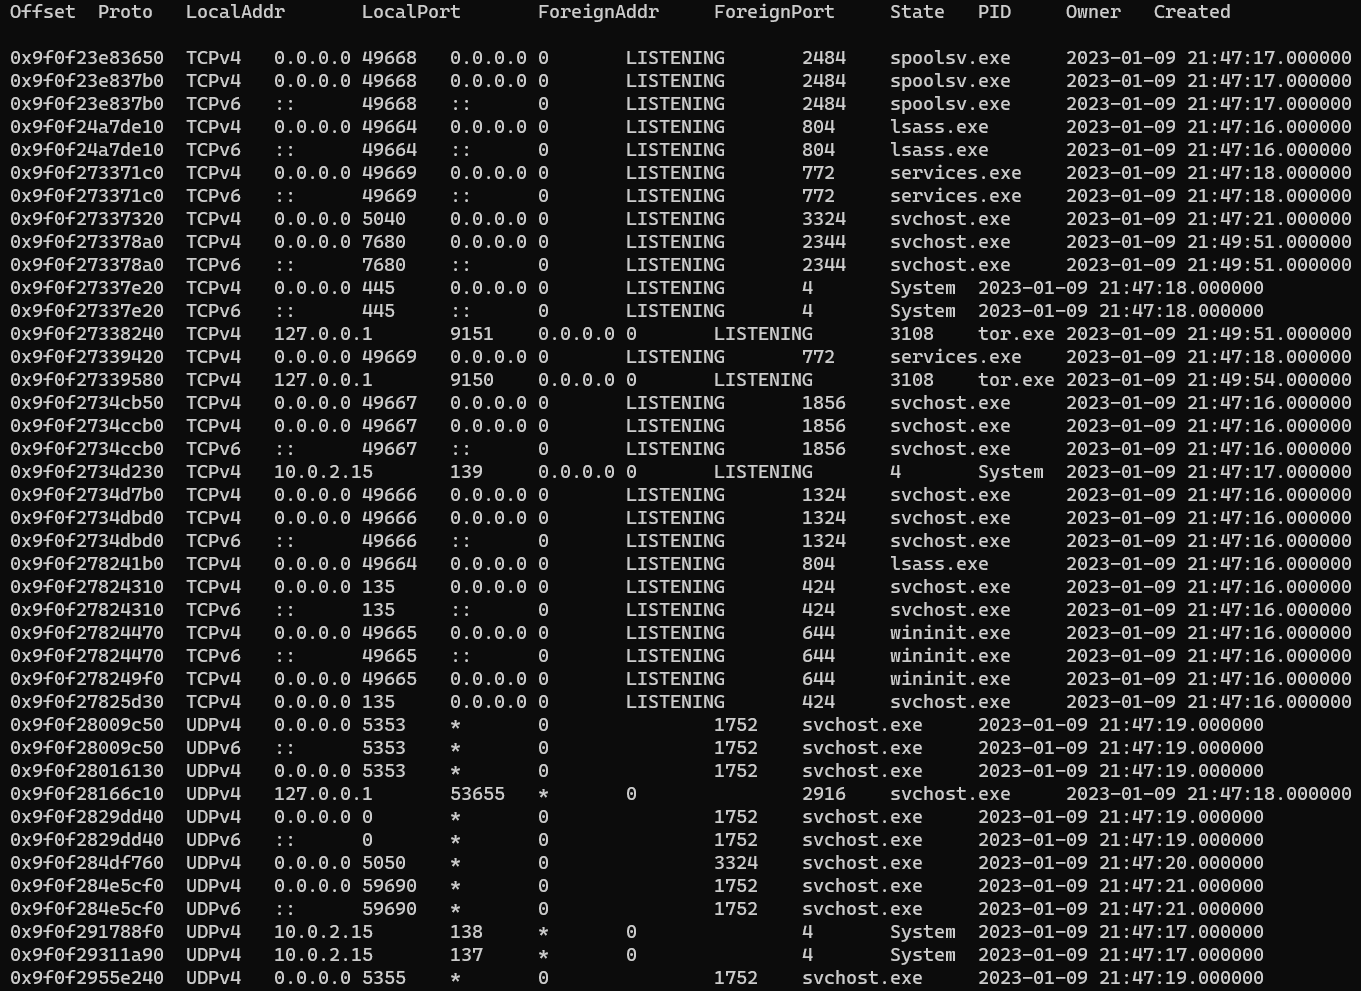
\includegraphics[width=\textwidth]{images/bobnet1.png}
        \end{subfigure}
        \begin{subfigure}[b]{\textwidth}
            \centering
                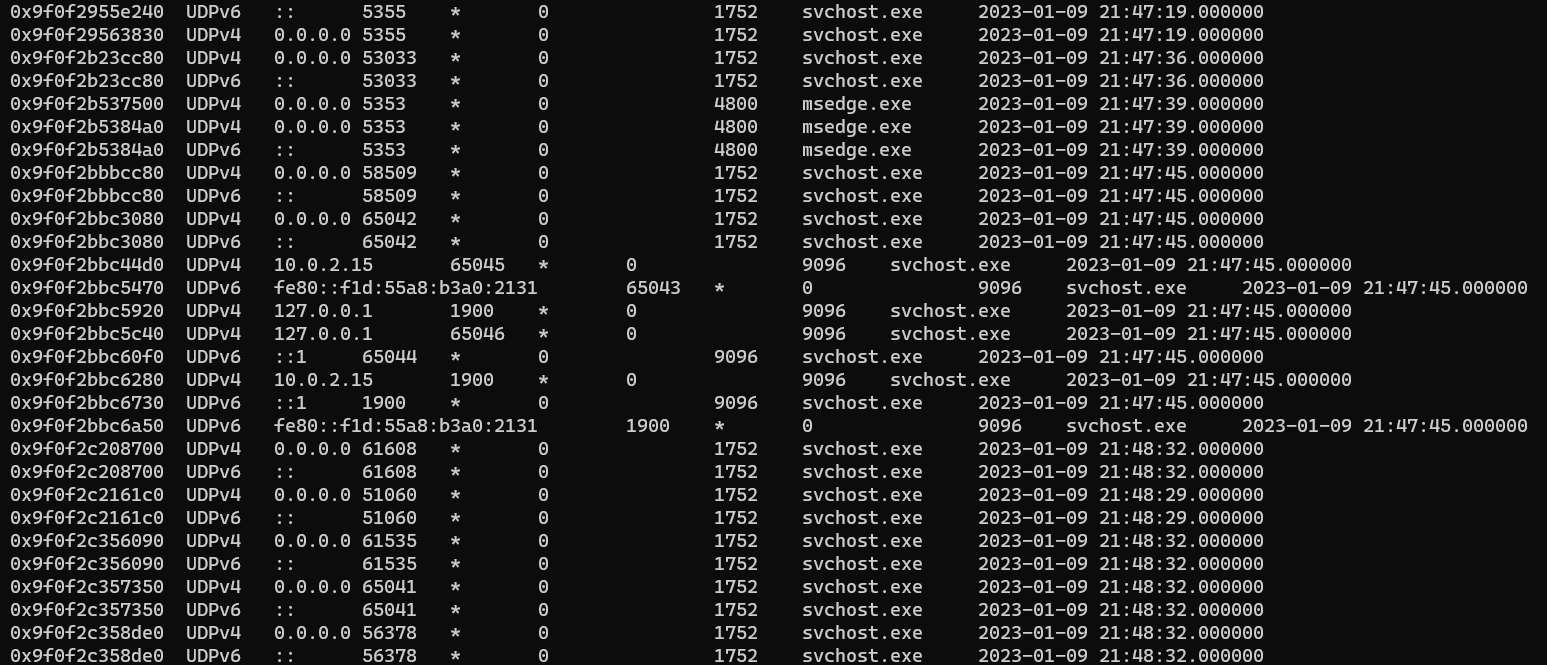
\includegraphics[width=\textwidth]{images/bobnet2.png}
        \end{subfigure}
        \caption{Network connections.}
        \label{fig:bobnet}
\end{figure}

\subsubsection{SID}

I looked for the SIDs: you can see some of them in Figure \ref{fig:sid}.

\begin{figure}
        \centering
        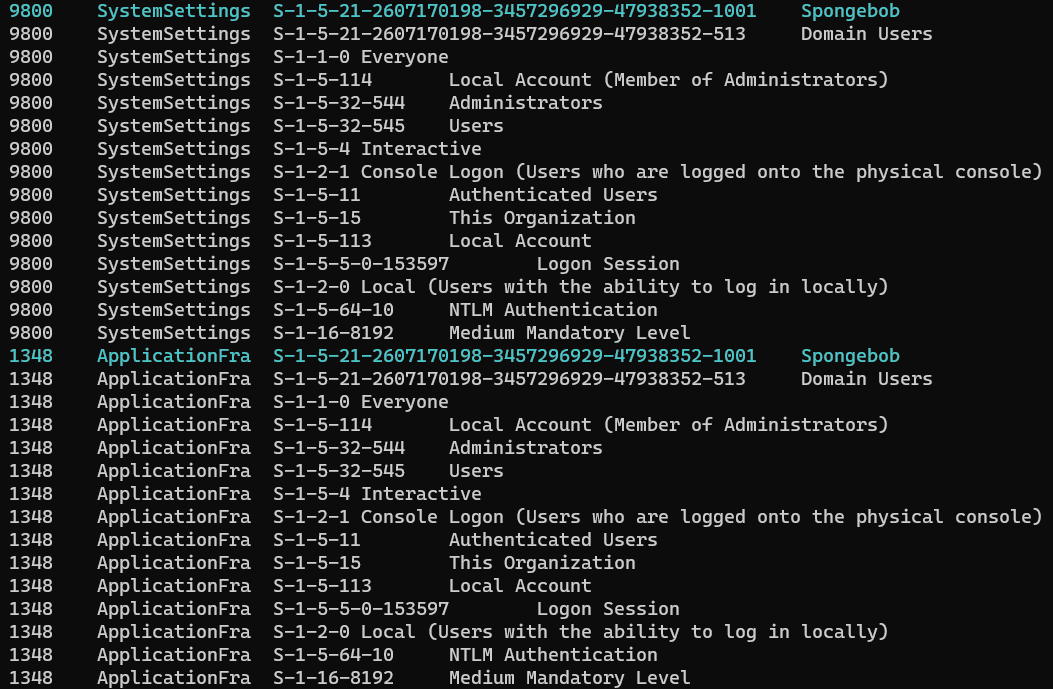
\includegraphics[width=\textwidth]{images/sids.png}
        \caption{SID of the user.}
        \label{fig:sid}
\end{figure}

\section{Expert testimony}

Observing the information about the RAM dump, we can retrieve the time of the dump, which is \textbf{2023-01-09 22:17:11}.

Taking a closer look to the running processes, we see that not all the browsers are the same. In fact, we have \textbf{msedge.exe} and \textbf{firefox.exe}. This means that the user was using two different browsers at the time of the dump.

I could also find the SID of the user, which is \textbf{S-1-5-21-2607170198-3457296929-47938352-1001}. This SID is associated to the user \textbf{Spongebob}.

\subsection{User password}

To retrieve the user password, I first got the hashes contained in the memory dump, then I used an online tool (hashes.com \cite{hashes}) to crack the hash: this tool searches for the hash in a database of already cracked hashes.

The hash is \texttt{bcf8548eae42900beda0f150e16504b5} and the associated password is: \\\texttt{ThisIsPatrick}.

Given this, we can assume that who sent the RAM dump is \textbf{Patrick}.

\addcontentsline{toc}{chapter}{References}
\printbibliography[title={References}]

\end{document}